\begin{tcolorbox}[posterbox]
\SectionTitle{N1 Cardinality Scaling}
\SmallText
\begin{itemize}
  \item Replicating prior passive findings, posterior N1 over POT scaled with small-number cardinality ($1 < 2 < 3$).
  \item Increasing changes elicited larger N1 amplitudes than Decreasing changes.
  \item N1 and P1--N1 peak-to-peak patterns grew with numerical distance in both directions.
\end{itemize}

\begin{center}
\begin{tabular}{c}
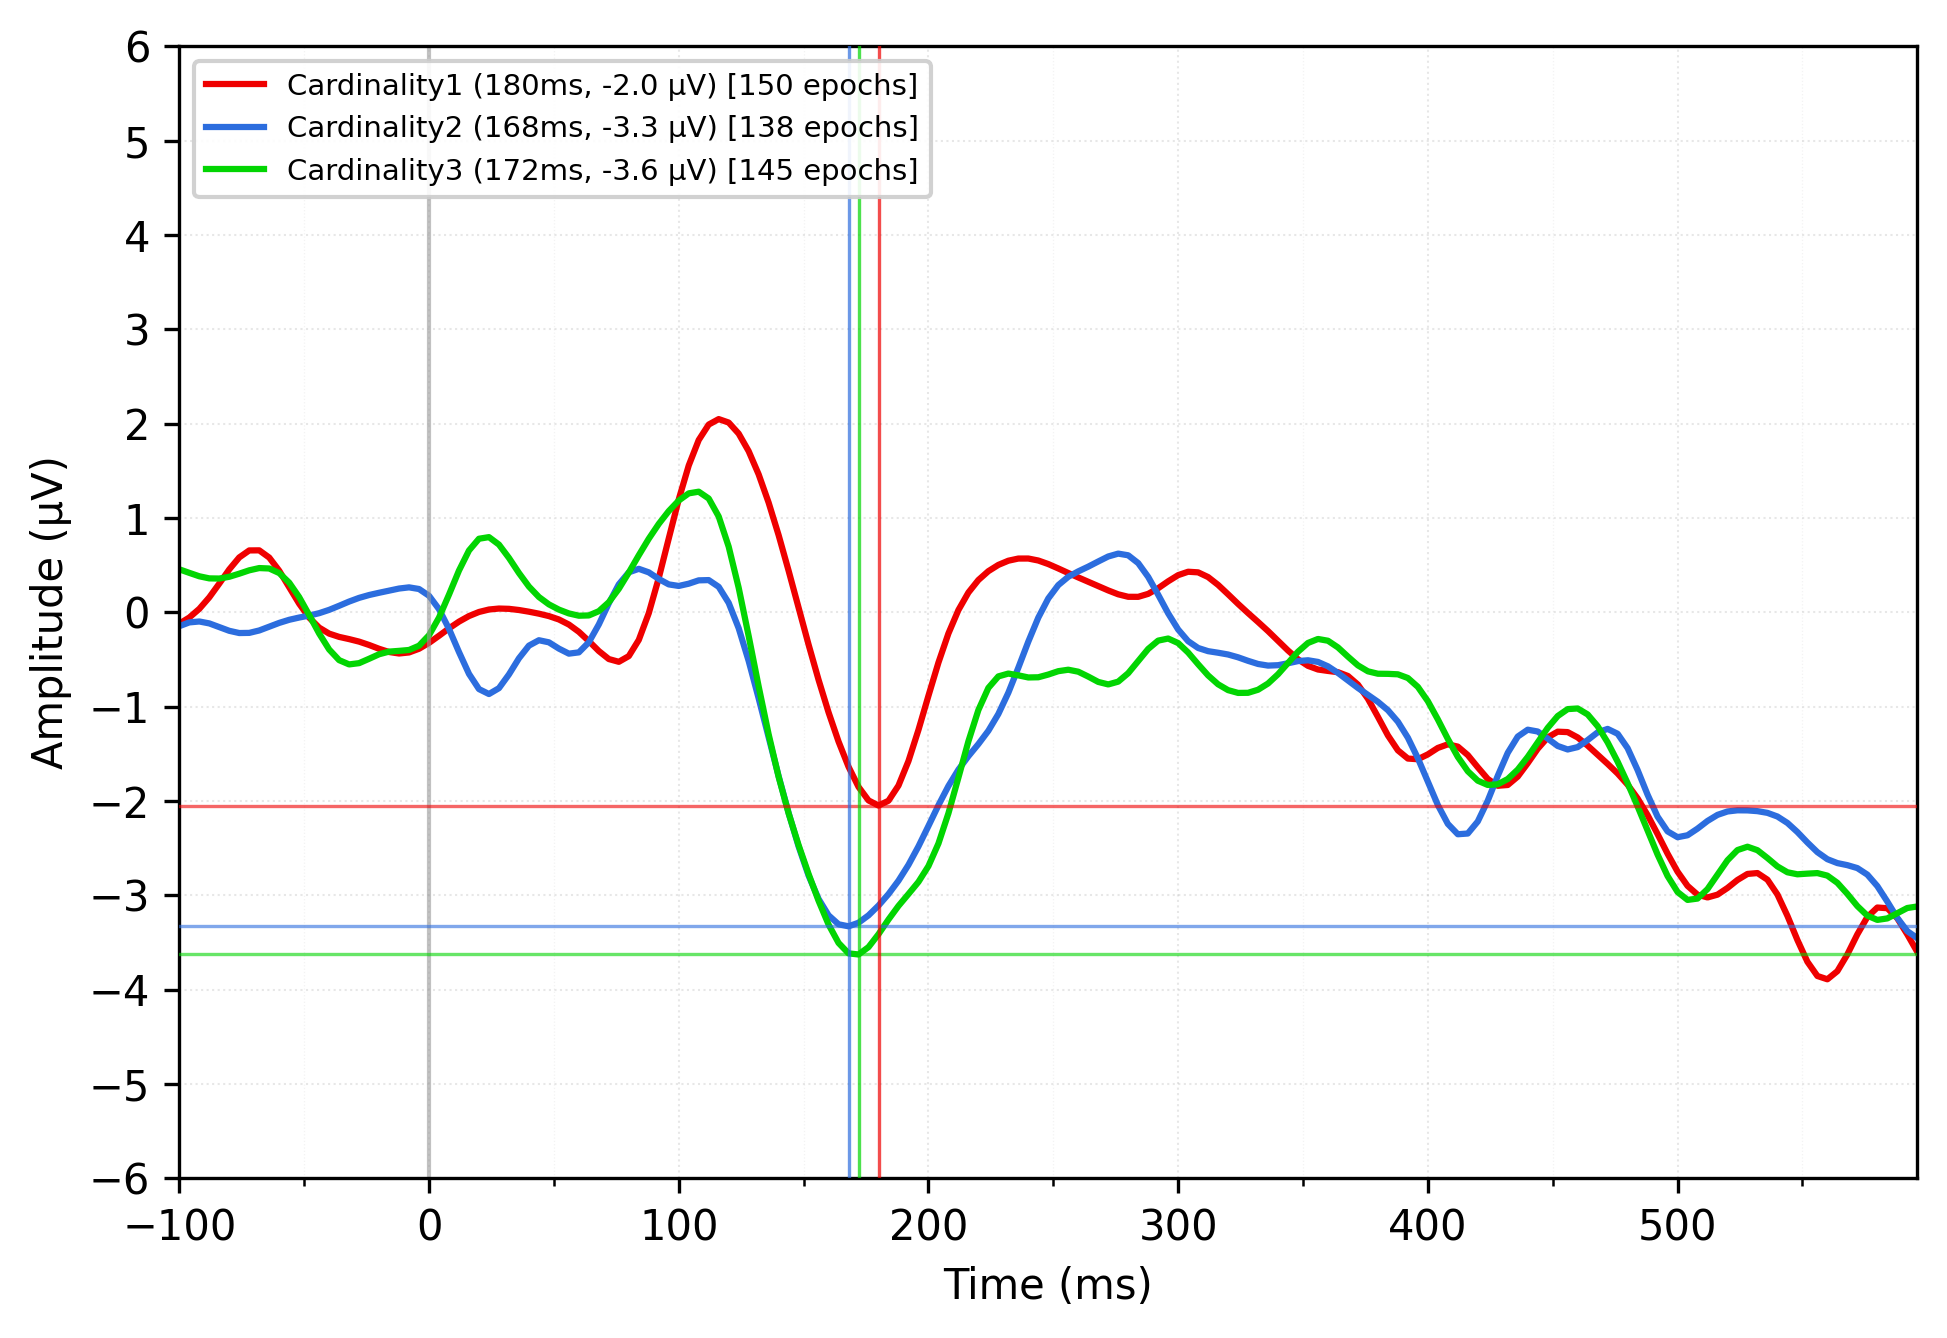
\includegraphics[width=0.86\linewidth, height=7in, keepaspectratio]{../docs/assets/plots/cardinality_within_small/cardinality_within_small-N1-no_topo.png} \\
[0.06em]
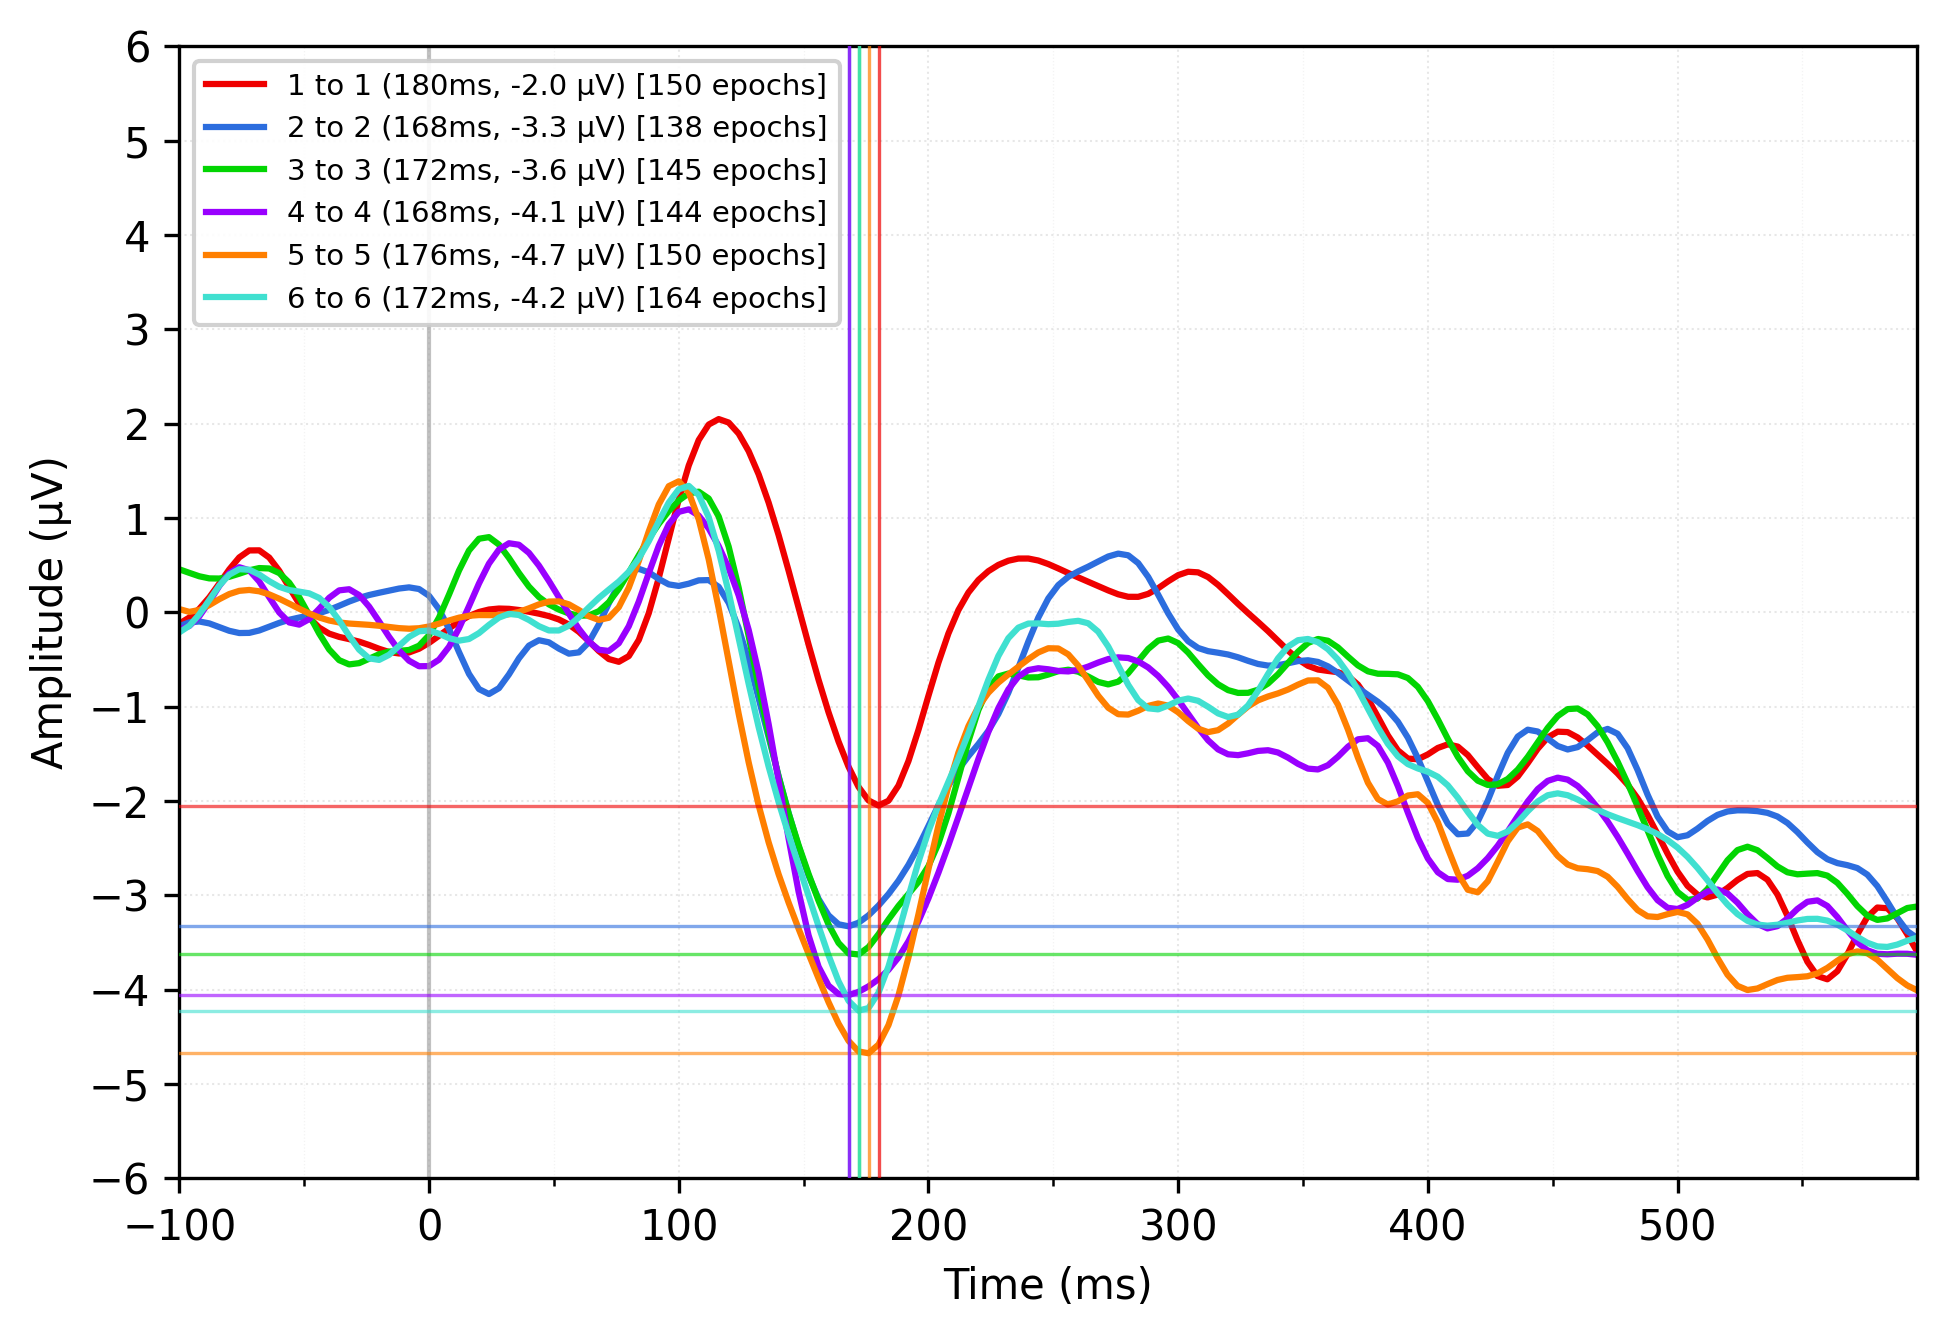
\includegraphics[width=0.86\linewidth, height=7in, keepaspectratio]{../docs/assets/plots/cardinality_all/cardinality_all-N1-no_topo.png} \\
\end{tabular}
\end{center}
\SmallText
\textbf{Fig. 5.} N1 no-topo overlays for cardinality scaling.
\end{tcolorbox}

\vspace{0.06in}

\begin{tcolorbox}[posterbox]
\SectionTitle{P3b: Working Memory Updating}
\SmallText
\begin{itemize}
  \item P3b peaked $\sim$460--480~ms over parietal (Pz); \textbf{Decreasing elicited larger P3b} than Increasing---mirroring the MMN direction asymmetry.
  \item P3b was markedly larger for change vs.\ no-change ($\sim$3.1 vs.\ 0.5~$\mu$V), confirming working memory engagement upon numerosity change.
\end{itemize}

\begin{center}
  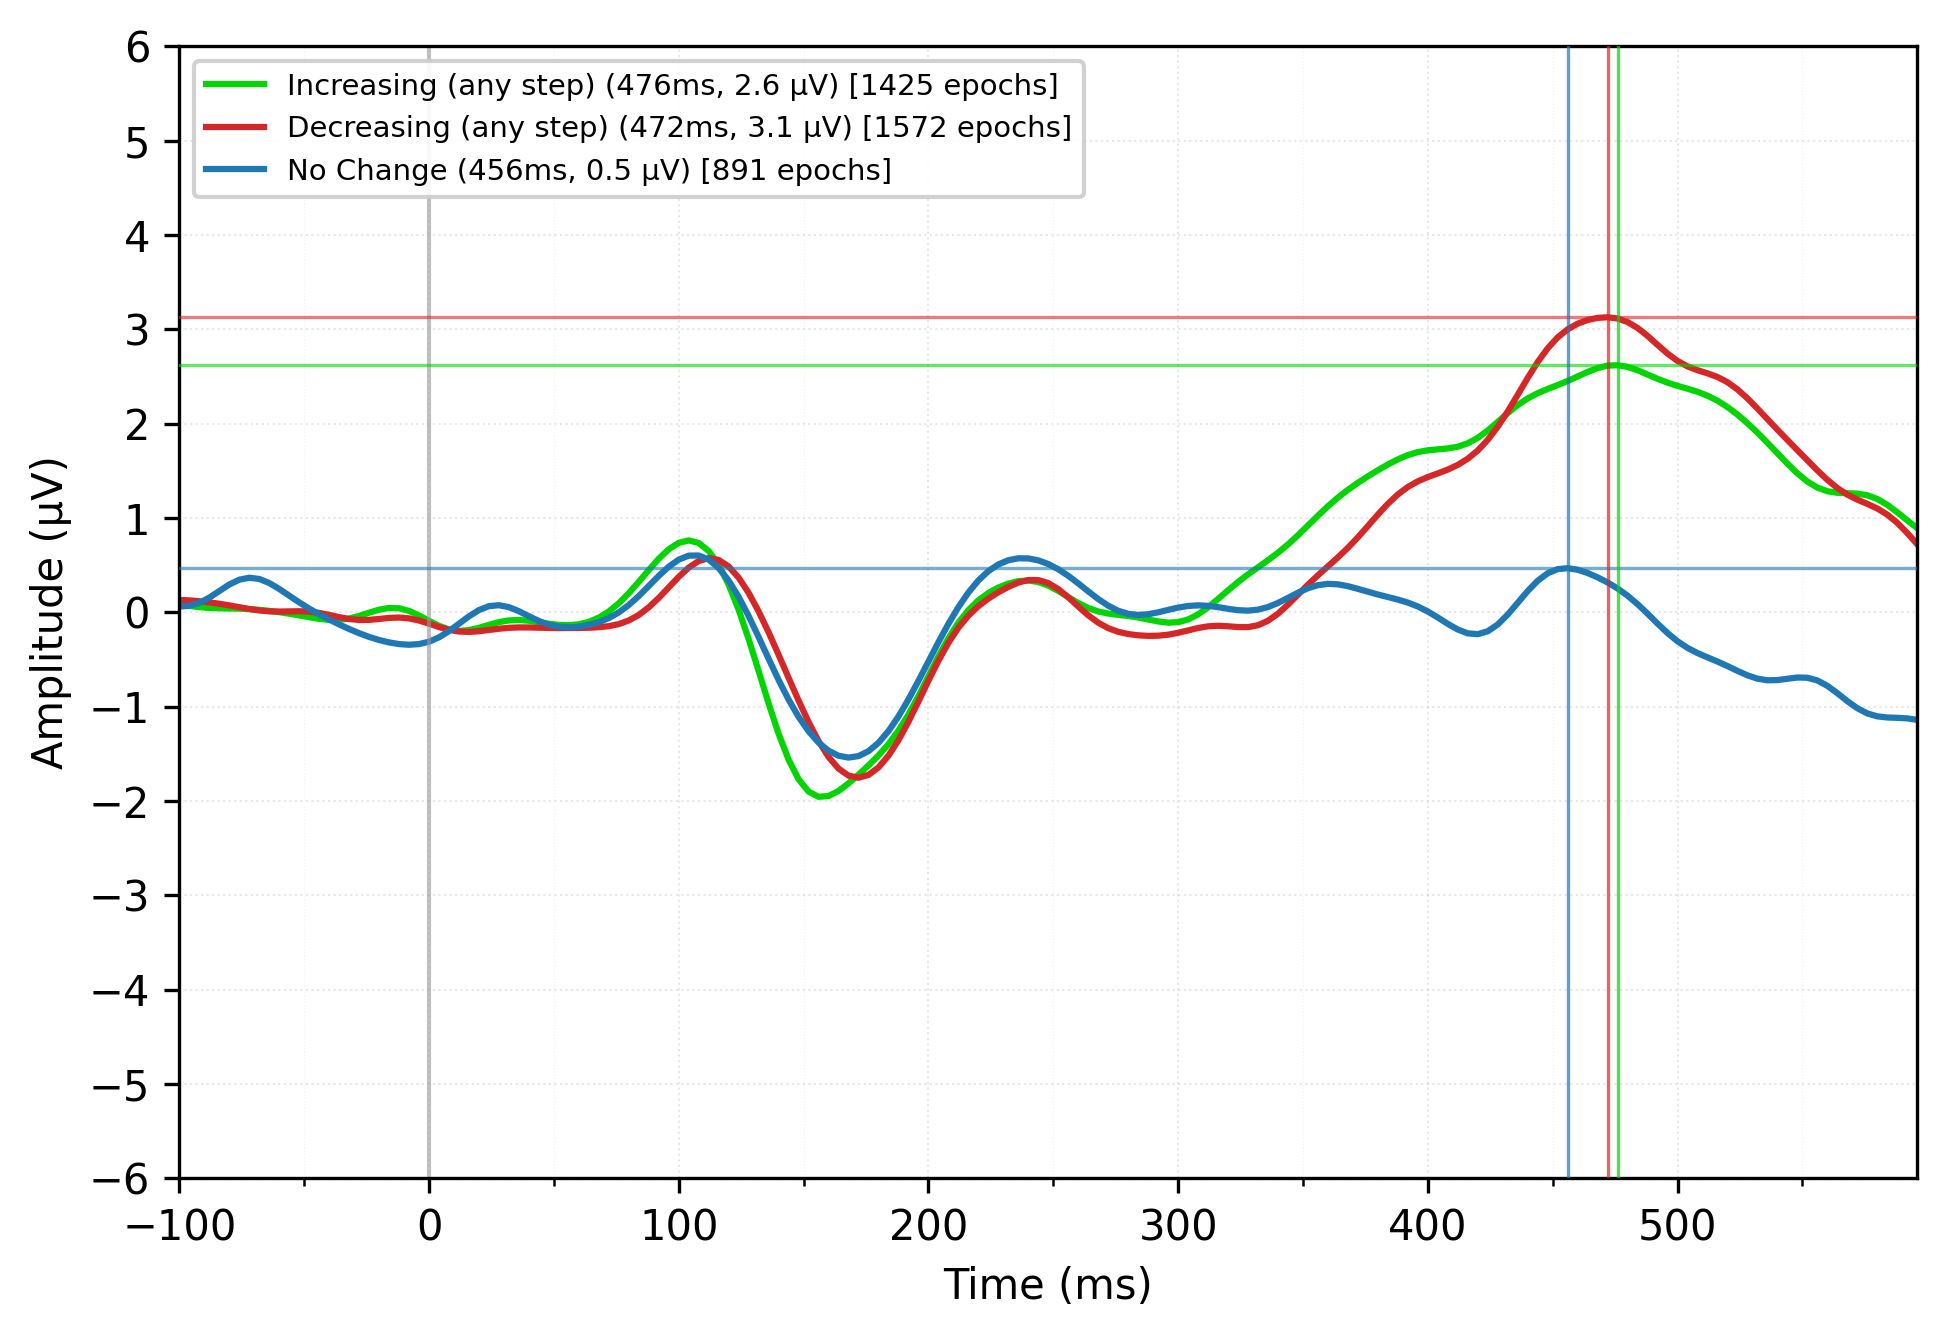
\includegraphics[width=0.86\linewidth, height=6in, keepaspectratio]{../docs/assets/plots/increase_decrease_cardinality_ACC1/increase_decrease_cardinality_ACC1-P3b-no_topo.png}
\end{center}
\SmallText
\textbf{Fig. 6.} P3b no-topo: direction effect and change vs.\ no-change (parietal Pz).
\end{tcolorbox}

\vfill

\begin{tcolorbox}[posterbox]
\SectionTitle{Conclusions}
\SmallText
\begin{itemize}
  \item \textbf{Active vs.\ Passive:} Active numerosity monitoring recruits rapid frontal mechanisms (MMN) distinct from posterior sensory processing (N1).
  \item \textbf{Direction Matters:} The brain processes increases and decreases of quantity differently.
  \item \textbf{Decreasing advantage:} Decreasing changes elicit higher accuracy and stronger frontal error signals (MMN).
  \item \textbf{Distance Effect:} Neural error signals scale with the magnitude of numerical change, mirroring behavioral performance.
  \item \textbf{Frontal/Posterior Dissociation:} Increasing changes drive larger posterior N1; Decreasing changes drive stronger frontal MMN---revealing dual neural processing streams for numerical change.
\end{itemize}
\end{tcolorbox}

\vspace{0.06in}

\begin{tcolorbox}[posterbox]
\SectionTitle{References}
{\fontsize{20}{24}\selectfont
\begin{itemize}
  \item Hyde, D.\,C., \& Spelke, E.\,S. (2012). \textit{Human Brain Mapping, 33}(9), 2189--2203.
  \item Gordon, P. (1994). ESSP, Paris, France.
  \item Polich, J. (2007). \textit{Clinical Neurophysiology, 118}(10), 2128--2148.
  \item Polich, J. (2011). In Kappenman \& Luck (Eds.), \textit{Oxford Handbook of ERP Components}.
  \item Temple, E., \& Posner, M.\,I. (1998). \textit{PNAS, 95}(13), 7836--7841.
\end{itemize}
}
\end{tcolorbox}
